\documentclass[12pt,letterpaper]{beamer}
\usetheme{Copenhagen}
\usecolortheme{seahorse}
\setbeamertemplate{section in toc}{\inserttocsection}

\usepackage[utf8]{inputenc}
\usepackage{amsmath}
\usepackage{amsfonts}
\usepackage{amssymb}
\usepackage{graphicx}
\graphicspath{ {./images/} }
\usepackage{multirow}
\usepackage{hyperref}
\hypersetup{
    colorlinks=true,
    linkcolor=blue,
    filecolor=magenta,      
    urlcolor=cyan,
    pdftitle={Overleaf Example},
    pdfpagemode=FullScreen,
}
\title[Robotics I]
{ENGR 3421: ROBOTICS I}
\subtitle{GPIO}

\author[Zhang, Lin]
{Dr. Lin Zhang}
\institute[UCA] % (optional)
{
  Department of Physics and Astronomy\\
  University of Central Arkansas
}
\date[Robotics1 2021] % (optional)
{August 31, 2021}
\logo{
\includegraphics[height=1cm]{../images/uca_bear_logo.png}}


%End of title page configuration block
%------------------------------------------------------------

%------------------------------------------------------------
%The next block of commands puts the table of contents at the beginning of each section and highlights the current section:

\AtBeginSection[]
{
  \begin{frame}
    \frametitle{Outline}
    \tableofcontents[currentsection]
  \end{frame}
}
%------------------------------------------------------------

\begin{document}

%The next statement creates the title page.
\frame{\titlepage}

%---------------------------------------------------------
%This block of code is for the table of contents after the title page
\begin{frame}
\frametitle{Outline}
\tableofcontents
\end{frame}
%---------------------------------------------------------


\section{Python Review}

\begin{frame}{Variables}
    \begin{itemize}
        \item a variable can store anything: number, list, object,...
        \item Use "=" to feed contents to a variable
    \end{itemize}
\end{frame}

\begin{frame}{Conditions}
    \begin{itemize}
        \item Use a boolean condition for your loop.
        \item $">", "<=", "==", "!="$ 
        \item "and", "or", "not", "is"
    \end{itemize}
\end{frame}

\begin{frame}{Assignment Hints}
    \begin{itemize}
        \item 1 "while" loop takes care of things happened in 0.02 seconds.
        \item Either set the LED brightness with a specific duty cycle or make it a constant.
        \item Read \href{https://gpiozero.readthedocs.io/en/stable/}{gpiozero} documentations, implement some \href{https://gpiozero.readthedocs.io/en/stable/recipes.html}{recipes}.
    \end{itemize}
\end{frame}

\section{PWM}

\begin{frame}{Pulse Width Modulation}
    \begin{columns}
        \column{0.5\textwidth}
        \begin{figure}
            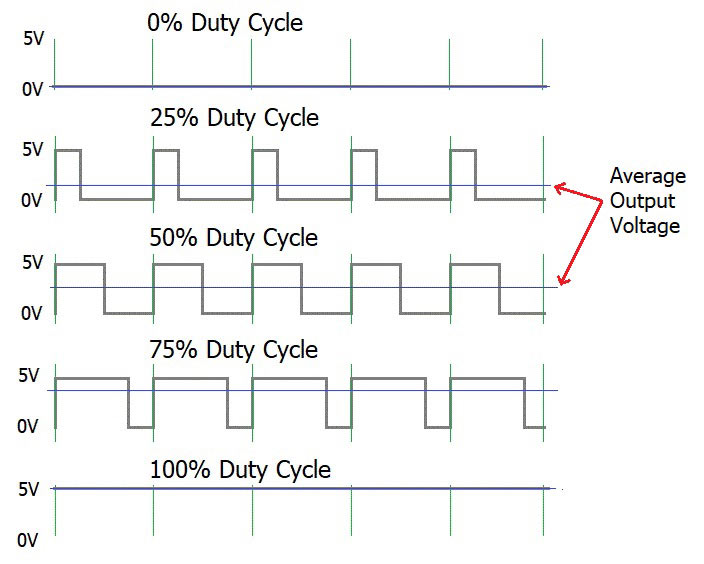
\includegraphics[width=0.9\textwidth]{pwm}
        \end{figure}

        \column{0.5\textwidth}
        {\scriptsize
            \begin{itemize}
                \item Simulate analogue signal with digital signal.
                \item Frequency controls continuity.
                \item Duty cycle controls signal strength. 
            \end{itemize}
        }

    \end{columns}

\end{frame}

\begin{frame}{Hardware PWM \& Software PWM}
    \begin{itemize}
        \item Fully hardware PWM 
            \begin{itemize}
                \item The most accurate and possibly the most flexible.
                \item Only available on GPIO 12/18 or GPIO 13/19.
            \end{itemize}
        \item DMA (Direct Memory Access) timed PWM.
            \begin{itemize}
                \item Intermediate accuracy but not flexible.
                \item Available on all GPIO pins.
            \end{itemize}
        \item Software timed PWM.
            \begin{itemize}
                \item The timing accuracy will vary but very flexible.
                \item Available on all GPIO pins.
                \item Not good for servos.
            \end{itemize}
        \item May require installation of \href{https://abyz.me.uk/rpi/pigpio/}{pigpio} library.
    \end{itemize}
\end{frame}
    
\section{Motor Driver}

\begin{frame}{Motor Driver}
    \begin{figure}
        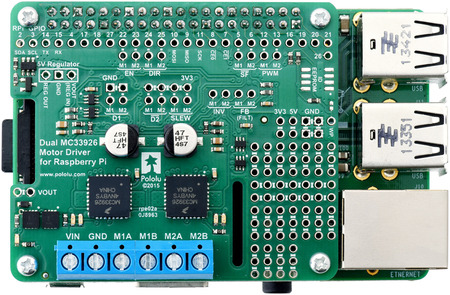
\includegraphics[width=0.47\textwidth]{driver_board}
        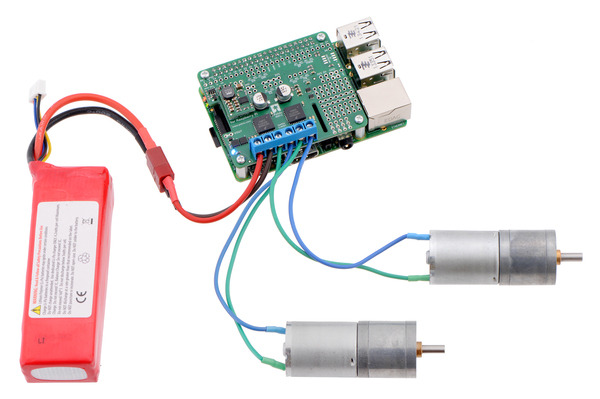
\includegraphics[width=0.47\textwidth]{driving_motors}
    \end{figure}
\end{frame}

\begin{frame}{Pin Mappings}
    % \begin{tabularx}{0.9\linewidth} { 
            % | >{\raggedright\arraybackslash}X 
            % | >{\centering\arraybackslash}X 
        % | >{\raggedleft\arraybackslash}X | }
        % \hline
        % GPIO Pin & Motor Driver Pin & Description \\
        % \hline
        % 5  & Motor 1 $\overline{SF}$  & Status flag output  \\
        % \hline
        % 6  & Motor 2 $\overline{SF}$  & Status flag output  \\
        % \hline
        % 12  & Motor 1 PWM  & Motor speed input, max PWM frequency: 20kHz  \\
        % \hline
        % 13  & Motor 2 PWM  & Motor speed input, max PWM frequency: 20kHz  \\
        % \hline
        % 22  & Motor 1 EN  & Enable input  \\
        % \hline
        % 23  & Motor 2 EN  & Enable input  \\
        % \hline
        % 24  & Motor 1 DIR  & Motor direction input. LOW: A to B; HIGH: B to A.  \\
        % \hline
        % 25  & Motor 2 DIR  & Motor direction input. LOW: A to B; HIGH: B to A.  \\
        % \hline
    % \end{tabularx}
    \begin{tabular}{ ccc }
        \hline
        GPIO Pin & Motor Driver Pin & Description \\
        \hline
        5  & Motor 1 $\overline{SF}$  & \multirow{2}{12em}{\scriptsize Status flag output}  \\
        6  & Motor 2 $\overline{SF}$  &  \\
        \hline
        12  & Motor 1 PWM  & \multirow{2}{12em}{\scriptsize Motor speed input, max PWM frequency: 20kHz}  \\
        13  & Motor 2 PWM  &  \\
        \hline
        22  & Motor 1 EN  & \multirow{2}{12em}{\scriptsize Enable input}  \\
        23  & Motor 2 EN  &  \\
        \hline
        24  & Motor 1 DIR  & \multirow{2}{12em}{\scriptsize Motor direction input. LOW: A to B; HIGH: B to A.}  \\
        25  & Motor 2 DIR  &  \\
        \hline
    \end{tabular}
\end{frame}

\begin{frame}{Python Library for Motor Driver}
    Check \href{https://github.com/linzhangUCA/dual-mc33926-motor-driver-rpi}{this repo} for installation instructions.
    \begin{block}{Note}
        Changes were made due to Python 3 compatibility. If using following original instructions, substitute $python$ with $python3$ and $pip$ with $pip3$
    \end{block}
\end{frame}

\begin{frame}{Soldering}
    \begin{alertblock}{Warning}
        Better get yourselves prepared with the practicing kits.
    \end{alertblock}
\end{frame}

\end{document}
